\documentclass[a4paper, 12pt]{article}
\usepackage{fancyhdr}
\usepackage{extramarks}
\usepackage{amsmath}
\usepackage{amsthm}
\usepackage{amsfonts}
\usepackage{booktabs} 
\usepackage{blindtext} 
\usepackage{graphicx}
\usepackage{longtable} 
\usepackage{tikz}
\usepackage[plain]{algorithm}
\usepackage{algpseudocode}
\usepackage{pgfplots}
\usepackage{hyperref} 
\usetikzlibrary{automata,positioning}

%
% Basic Document Settings
%

\topmargin=-0.45in
\evensidemargin=0in
\oddsidemargin=0in
\textwidth=6.5in
\textheight=9.0in
\headsep=0.25in

\linespread{1.1}

\pagestyle{fancy}
\lhead{\hmwkAuthorName}
\chead{\hmwkTitle}
\rhead{\hmwkClass}
\lfoot{\lastxmark}
\cfoot{\thepage}

%
% Create Problem Sections
%

% Homework Problem Environment
%
% This environment takes an optional argument. When given, it will adjust the
% problem counter. This is useful for when the problems given for your
% assignment aren't sequential. See the last 3 problems of this template for an
% example.
%

% Homework Details
%   - Title
%   - Due date
%   - Class
%   - Section/Time
%   - Instructor
%   - Author
%

\newcommand{\hmwkTitle}{Stock Market Challenge}
\newcommand{\hmwkDueDate}{2024, December 19}
\newcommand{\hmwkClass}{CIA4U}
\newcommand{\hmwkClassTime}{Period C}
\newcommand{\hmwkClassInstructor}{Mr. David Warrener}
\newcommand{\hmwkAuthorName}{\textbf{Gregory Polstvin}}

%
% Title Page
%

\title{
    \vspace{2in}
    \textmd{\textbf{\hmwkClass:\ \hmwkTitle}}\\
    \normalsize\vspace{0.1in}\small{Due\ on\ \hmwkDueDate\ at 12:00}\\
    \vspace{0.1in}\large{\textit{\hmwkClassInstructor\ \hmwkClassTime}}
    \vspace{3in}
}

\author{\hmwkAuthorName}
\date{}


\graphicspath{ {~/Downloads} }

\begin{document}
\maketitle
\pagebreak
\tableofcontents
\pagebreak

\section{Trading Activity and Performance}%
\begin{longtable}{|l|l|l|r|r|r|}
\hline
\textbf{Date} & \textbf{Transaction Type} & \textbf{Symbol} & \textbf{QTY} &
\textbf{Price (USD)} & \textbf{Gains/Losses (USD)} \\ \hline
12/02/2024  & Buy        & SMCI  & 100   & 42.30   & -4,230.00    \\ \hline
12/02/2024  & Sell       & GOOG  & -650  & 172.88  & 112,372.00   \\ \hline
11/20/2024  & Sell       & APLS  & -3000 & 28.13   & 84,390.00    \\ \hline
11/19/2024  & Buy        & APLS  & 3000  & 30.23   & -90,690.00   \\ \hline
11/19/2024  & Buy        & SMCI  & 3000  & 28.30   & -84,900.00   \\ \hline
11/19/2024  & Sell       & LMT   & -150  & 533.11  & 79,966.50    \\ \hline
11/19/2024  & Sell       & PDD   & -632  & 117.15  & 74,038.80    \\ \hline
11/18/2024  & Sell       & SHOP  & -500  & 107.58  & 53,790.00    \\ \hline
11/15/2024  & Dividends  & HON   & 360   & 1.13    & 406.80      \\ \hline
11/12/2024  & Buy        & DAL   & 338   & 63.49   & -21,459.62   \\ \hline
11/12/2024  & Sell       & BABA  & -190  & 91.88   & 17,457.20    \\ \hline
11/12/2024  & Buy        & SHOP  & 500   & 113.02  & -56,510.00   \\ \hline
11/12/2024  & Sell       & MULN  & -20000 & 3.00   & 6,0000.00    \\ \hline
11/12/2024  & Buy        & MULN  & 20000 & 3.04    & -60,800.00   \\ \hline
11/12/2024  & Sell       & BABA  & -660  & 91.67   & 60,502.20    \\ \hline
10/31/2024  & Buy        & PDD   & 632   & 118.50  & -74,892.00   \\ \hline
10/29/2024  & Buy        & HON   & 360   & 206.95  & -74,502.00   \\ \hline
10/29/2024  & Buy        & DAL   & 1250  & 56.22   & -70,275.00   \\ \hline
10/29/2024  & Buy        & GOOG  & 650   & 170.17  & -110,610.50  \\ \hline
10/29/2024  & Buy        & LMT   & 150   & 551.06  & -82,659.00   \\ \hline
10/29/2024  & Buy        & BABA  & 850   & 100.26  & -85,221.00   \\ \hline
\end{longtable}

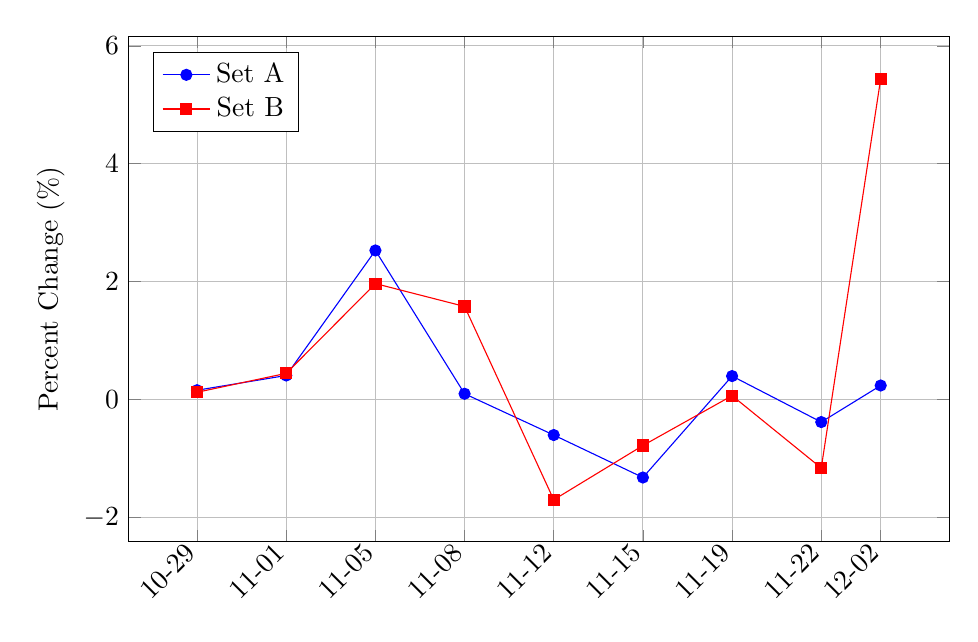
\begin{tikzpicture}
    \begin{axis}[
        ylabel={Percent Change (\%)},
        xtick={0, 3, 6, 9, 12, 15, 18, 21, 23},
        xticklabels={10-29,11-01,11-05,11-08,11-12,11-15,11-19,11-22,12-02},
        xticklabel style={rotate=45, anchor=east},
        legend pos=north west,
        grid=major,
        width=12cm,
        height=8cm,
    ]
        % Set A
        \addplot[mark=*,blue] coordinates {
            (0, 0.16)
            (3, 0.41)
            (6, 2.53)
            (9, 0.1)
            (12, -0.6)
            (15, -1.32)
            (18, 0.4)
            (21, -0.38)
            (23, 0.24)
        };
        \addlegendentry{Set A}
        
        % Set B
        \addplot[mark=square*,red] coordinates {
            (0, 0.12536)
            (3, 0.44633338721200566)
            (6, 1.9677942056038233)
            (9, 1.5802936059640116)
            (12, -1.6978442451378917)
            (15, -0.7778339503048293)
            (18, 0.06755858900493461)
            (21, -1.1592440349965982)
            (23, 5.443545172584208)
        };
        \addlegendentry{Set B}
    \end{axis}
\end{tikzpicture}

\subsection{Portfolio: Open Positions, Balances, and Performance}%

\begin{longtable}{|l|l|l|l|l|l|}
\hline
\textbf{Symbol} & \textbf{QTY} & \textbf{Paid} & \textbf{Last Price} & \textbf{Mrkt. Value} & \textbf{Profit} \\ \hline
\textbf{DAL} & 1,588 & 57.77 & 63.41 & \$100,695.08 & \$8,960.46 (9.77\%) \\
\hline
\textbf{HON} & 360 & 206.95 & 229.95 & \$82,782.00 & \$8,280.00 (11.11\%) \\
\hline
\textbf{SMCI} & 3,100 & 28.75 & 42.00 & \$130,200.00 & \$41,070.00 (46.08\%) \\
\hline
\end{longtable}

% \includegraphics{sp500-perf}
% \includegraphics{open-pos}
\noindent
\textbf{Initial Cash: } \$500,000.00 \\
\textbf{Value:} \$539,651.46 (7.93\%) \\
\textbf{Cash Balance:} \$225,974.38 \\
\textbf{SPY ETF \% Return:} 4.25\% \\
\textbf{Portfolio Return:} 7.93\% \\

\section{Analysis of SMCI and Company}

Initially, I had plans to purchase the stock on October 29. However, I hesitated massively due to a 
class action lawsuit coming out against SMCI. The allegations stated that SMCI's representations 
about its business, operations, and prospects were either false, misleading, and/or lacked a 
reasonable basis at all relevant times. Consequently, the share price plummeted by over 40\%.

These allegations were serious enough to raise concerns about SMCI potentially being delisted 
from NASDAQ. Such a move would have been detrimental to the company, as liquidity and transparency 
would decrease massively. With their reputation already hanging by a thread, a delisting would likely 
have led to bankruptcy. \\

Despite these concerns, I purchased SMCI on November 19, after SMCI had put out a detailed report 
on how they plan on not getting delisted. This was in an effort to earn funds quickly within 
the shortest possible timeframe, a strategy not I would not advise to anyone.
Recognizing this as an incredibly risky move, I limited my investment to approximately 
85 thousand dollars. \\

Since then, bull run raised stock price up 48\% from the 19th to the 2nd, the final day of the challenge. Reflecting 
on this decision, it’s clear that my intuition played a significant role.  Drawing on my experiences (see \textit{On Trading}), 
I though I trusted my ability to analyze market overreactions and identify opportunities where others saw only risk. 
This was an incredibly reckless approach, as I took a gamble based on my
understanding of the stock market, ignoring recommended advice. \\

\section{Indicators of Other Best Companies}

These are my other best performing stocks.
I had initially went with my gut feeling for each of these stocks,
and I had affirmed my decisions using a reasonably simple algorithm.

\subsection{Analysis Algorithm} % (fold)

To start, I collected daily closing prices for time periods that best reflected
the market currently, using data from Yahoo Finance. When the adjusted 
closing price was unavailable, I substituted the standard closing price to 
maintain consistency. For the first day of data, I included the opening 
price in the returns calculation to ensure that the algorithm accurately 
reflected price movements from the 
initial moment of analysis. \\

I calculated daily logarithmic returns using the formula: \\
\[
\log (\frac{P_t}{P_t-1})
\] \\
where $P_t$ represents the day in question, providing a reasonably accurate
 representation of percentage changes and accounts for compounding effects. \\

Next, I calculated the mean ($\mu_c$) and standard deviation ($\sigma_c$) of
these daily returns as follows: \\
\[
    \mu_c = n \cdot \mu_d
\] \\
where $n$ is the number of trading days. $c$ represents cumulatice, and 
$d$ represents daily. \\

For the standard deviation: \\
\[
    \sigma_c = \sqrt{n} \cdot \sigma_d
\] \\
Using these cumulative statistics, I worked out the probability of a 10\% gain
by the end of the analysis period. (10\% was chosen as a realistic, although
ambitious goal, as I would consider it to be in an area that would best assess
risk to performance.) The threshold for this gain is defined as
a logarithm: \\
\[
    TS = \log(1.10) + log(P_o)
\] 

The probability was then derived using the cumulative distribution function
(CDF) of the normal distribution: \\
\[
    P(x > TS) = 1 - \Phi (\frac{TS - \mu_c}{\sigma_c})
\] \\

This allowed me to quantify the likelihood of achieving significant gains for
each stock. Through this algorithm, the chances of my stock achieving a 10\%
gain from my inital price produced the following results: \\
\begin{itemize}
    \item \textbf{DAL:} 47.14\%
    \item \textbf{HON:} 71.83\%
\end{itemize}

You can see how I implemented this on the Github repo for this assignment:
\url{https://github.com/gripols/cia4u-isu}

%%%%%%%%%%%%%%%%%%%%%%%%%%%%%%%%%%%%%%%%%

\subsection*{Honeywell (HON)}%
Honeywell (HON) in the past year has been incredibly 
stable, and has consistently met price targets each 
quarter. I purchased stock coinciding with a bear run, 
which presented itself a great time to buy. 

From October 29, 2024, to December 2, 2024, I worked out the the probability of HON achieving a 10\% gain was calculated to be approximately 71.83\%. As of December 2,
2024, a profit of 11.11\% has been realized.

\subsubsection*{Other Metrics}

Analyst's Recommendations: 2.5. Most analysts earlier in the year
had recommended that it was a hold. Since then, analysts found

Price-to-Earnings (P/E) Ratio: 25.43 \\

Dividend Yield: Around 2.18\%. \\

Revenue Growth: Honeywell reported revenue of \$36.90 billion 
over the trailing twelve months, showcasing its robust business operations. \\

%%%%%%%%%%%%%%%%%%%%%%%%%%%%%%%%%%%%%%%%%

\subsection*{Delta Airline (DAL)}% FINISH THIS

Since 2008, the "Big Four" U.S. airline stocks (Delta, Southwest, 
American Airlines, and United) have delivered an average gain of 13.6\%, 
with the top performer, Delta, delivering an average gain of 20.8\% within two months.
This made Delta an incredibly attractive investment, especially in the span 
of this challenge. With a price-to-earnings (P/E) ratio of 7.14, 
I made the move to purchase it.\\

Upon my own analysis, Delta's probability of achieving a 10\% gain 
was calculated as 47.13\%. However, given past growth, I strongly 
believed that the real growth rate would be higher. 

\subsubsection*{Analyst Recommendation}


\subsubsection*{Other Metrics}
\begin{itemize}
    \item Price-to-Earnings (P/E) Ratio: Approximately 7.14, suggesting a 
    potentially undervalued stock relative to earnings.
    \item Dividend Yield: Delta Air Lines reinstated its dividend with a yield of around 0.85\%,
    which is quite cautious, but very safe.
    \item Revenue Growth: Delta reported revenue of \$58.05 billion over the 
    trailing twelve months, making Delta the largest airline in the world in terms of revenue.
\end{itemize}



%%%%%%%%%%%%%%%%%%%%%%%%%%%%%%%%%%%%%%%%%

\section{On Trading}

Prior to this challenge, from February to March of this year, 
I had participated in a highly active form of trading called day trading, 
focusing mostly on large, established cryptocurrencies, such as Bitcoin, 
and Ethereum. For 95\% of people, the logic behind it isn't so much strategy, 
as it is obfuscated gambling and following the crowd, as people approach
trading with incredibly high expectations, and will stop at nothing. \\

Despite this, I had made a return of over 60\% on my investments within the
span of a month, mostly focusing on Ethereum. While the financial results are
undeniably impressive, the experience itself is far from fulfilling. It's 
an incredibly mentally tiresome experience. You spend a lot of your time reading
news that ends up becoming useless and constantly monitoring price movements.
There's this looming sense of paranoia that looms with you, so even if you're doing
something fun, the question of "am I losing money right now?" is always on your mind. \\

Even with the returns I achieved, I can't shake the feeling that 
much of my success was due to luck rather than skill. \\

Through the challenge, I was forced to re-evaluate my approach to trading with the 15-minute delay on stocks purchased. I began to consider the positives of passive investing with the challenge, as I couldn't help but feel that my successes from day trading were from pure luck. \\

Reflecting on my experience from the challenge, I believe that IF I had the
money to invest, I would invest passively through a carefully managed ETF, 
since I don't think I would have the time or knowledge for managing my
investments, and I probably have better things to do at that point. 
However, at this stage in my life, passive investing doesn't feel practical.
I want access to my money when I need it, not just when the market opens on
Monday, and I don't have enough to realize any meaningful profits. \\

For those with the financial means, ETFs represent a far more 
stable and less stressful way to grow wealth over time. 
I welcome the benefits that come from such an approach, 
but it feels distant for me right now. I believe that's why
people are so drawn to day trading; that they feel like they could
make money quickly and be successful easily. At least, that's how I felt.\\ 
\end{document}
